\documentclass{article}

%\usepackage{lab}
%\usepackage[cn]{lab}
\usepackage[draft]{lab}


\newcommand{\AlgName}{YourAlgorithmName}


\begin{document}

%\tableofcontents

\section{\szxtitle{the first section as a simple test}}
\label{sec:s1}

\begin{szxitem}
	\item\textbf{first}
	the first item ...
	 
	\item\textbf{second}
	the second item ...
\end{szxitem}

\begin{szxenum}
	\item\textbf{first}
	the first enum ...
	
	\item\textbf{second}
	the second enum ...
\end{szxenum}

\begin{equation}
\label{equ:e1}
a+b=c
\end{equation}

\begin{equation}
\label{equ:e2}
a+b=c
\end{equation}

\begin{equation}
\label{equ:e3}
a+b=c
\end{equation}

\section{\szxtitle{the second section as another test}}
\label{sec:s2}

test1.

\szxoutline{outline1.}

test2.
\szxoutline{outline2.}

\szxoutline{outline2.}
There are some\szxadd{ things to add}.
There are some\szxdel{ words to delete}.


\begin{definition}
some definition.
\label{def:sample}
\end{definition}

\szxrefdef{def:sample} ...

\begin{proposition}
some proposition.
\label{prop:sample}
\end{proposition}
\begin{proof}
some proof.
\qedhere
\end{proof}

\szxrefprop{prop:sample} ...

\section{\szxtitle{the third section as another test}}
\label{sec:s3}

\szxrefsec{sec:s1}\\
\szxrefSec{sec:s1}\\
\szxrefsec{sec:s1,sec:s2}\\
\szxrefSecs{sec:s1,sec:s2}\\
\szxrefsec{sec:s1,sec:s2,sec:s3}\\
\szxrefSecs{sec:s1,sec:s2,sec:s3}\\

\szxrefequ{equ:e1}\\
\szxrefEqu{equ:e1}\\
\szxrefequs{equ:e1,equ:e2}\\
\szxrefEqus{equ:e1,equ:e2}\\
\szxrefequs{equ:e1,equ:e2,equ:e3}\\
\szxrefEqus{equ:e1,equ:e2,equ:e3}\\


\begin{szxalg}[!tb]
	\caption{\label{alg:framework}General framework of \AlgName{}}
	\KwIn{an instance $I$ of the SDVRP}
	\KwOut{the best solution $s^{*}$ found so far}
	$f^{*} \leftarrow +\infty$\;\label{line:init}
	\While{time limit is not met\label{line:term}}
	{
		\If{$f(s) < f^{*}_{iter}$\label{line:check}}
		{
			$f^{*}_{iter} \leftarrow f(s)$\;\label{line:update}
		}
		\Else
		{
			$stagnation \leftarrow stagnation + 1$\;
		}
	}
	return $s^{*}$\;
\end{szxalg}

\szxrefalg{alg:framework} ...
\szxrefline{line:init} ...
\szxrefline{line:init,line:update} ...
\szxrefline{line:term,line:check,line:update} ...

\begin{lstlisting}[language=json,caption={Sample configuration file.},label={code:cfg}]
{
  "random_seed": 42,
  "acceptance_rule": {
    "type": "LAHC",
  },
  "inter_operators": [
    [ "Relocate" ],
    [ "Swap<2, 0>", "Swap<2, 1>", "Swap<2, 2>" ]
  ],
  "intra_operators": [ "Exchange", "OrOpt<1>" ]
}
\end{lstlisting}

\szxrefcode{code:cfg} ...

\szxreffig{fig:columnwidth} illustrates ...
\szxreffig{fig:textwidth} illustrates ...
\szxreffig{fig:convergence2} illustrates ...

\begin{szxfig}[!tb]
	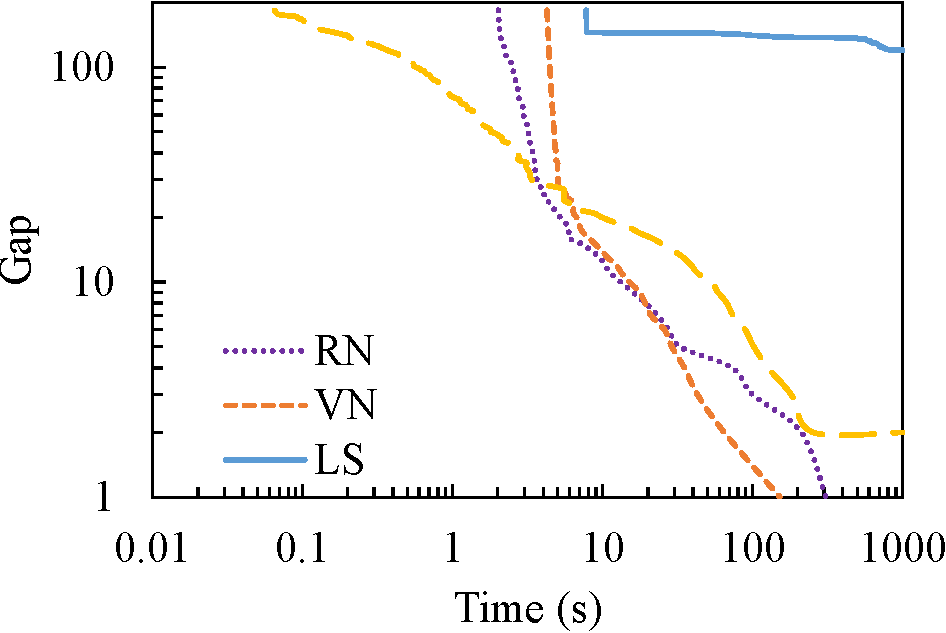
\includegraphics[width=0.5\columnwidth]{fig-SampleFigure.pdf}
	\caption{Evolution of the objective value gaps.}
	\label{fig:columnwidth}
\end{szxfig}


\begin{szxfig*}[!tb]
	\centering
	\begin{subfigure}[b]{0.31\textwidth}
		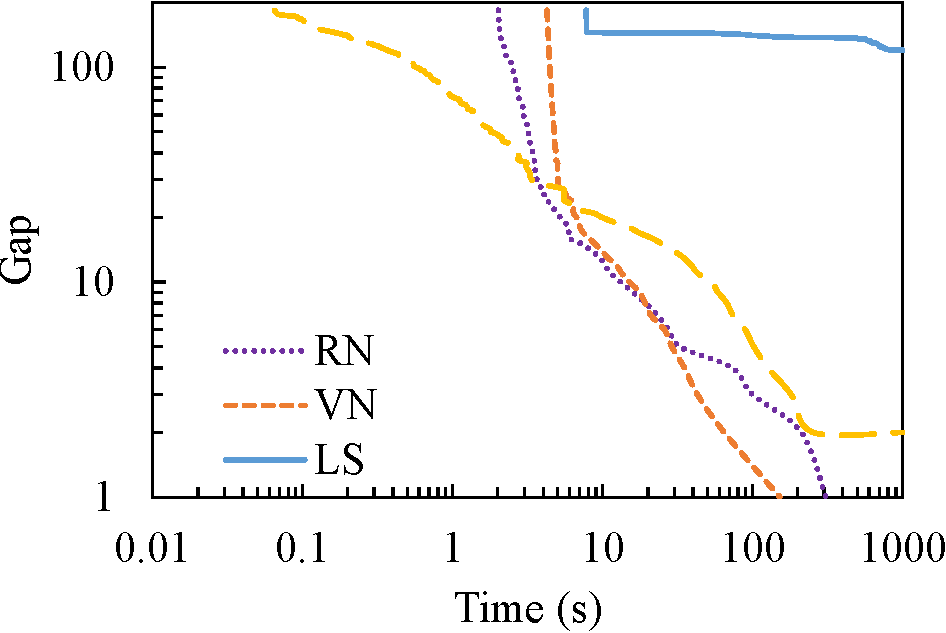
\includegraphics[width=\textwidth]{fig-SampleFigure.pdf}
		\caption{Plot1.}
		\label{fig:convergence1}
	\end{subfigure}
	~
	\begin{subfigure}[b]{0.31\textwidth}
		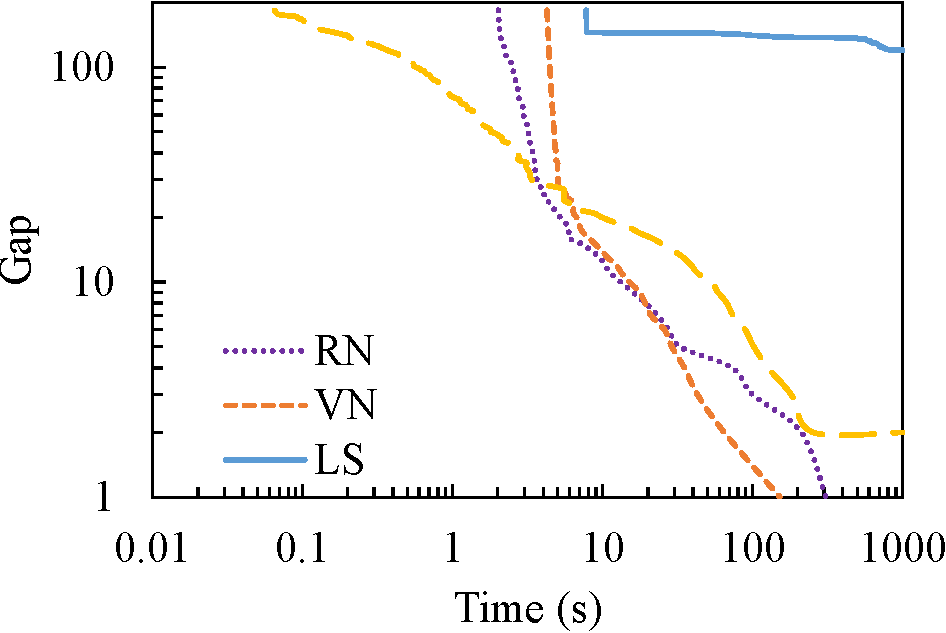
\includegraphics[width=\textwidth]{fig-SampleFigure.pdf}
		\caption{Plot2.}
		\label{fig:convergence2}
	\end{subfigure}
	~
	\begin{subfigure}[b]{0.31\textwidth}
		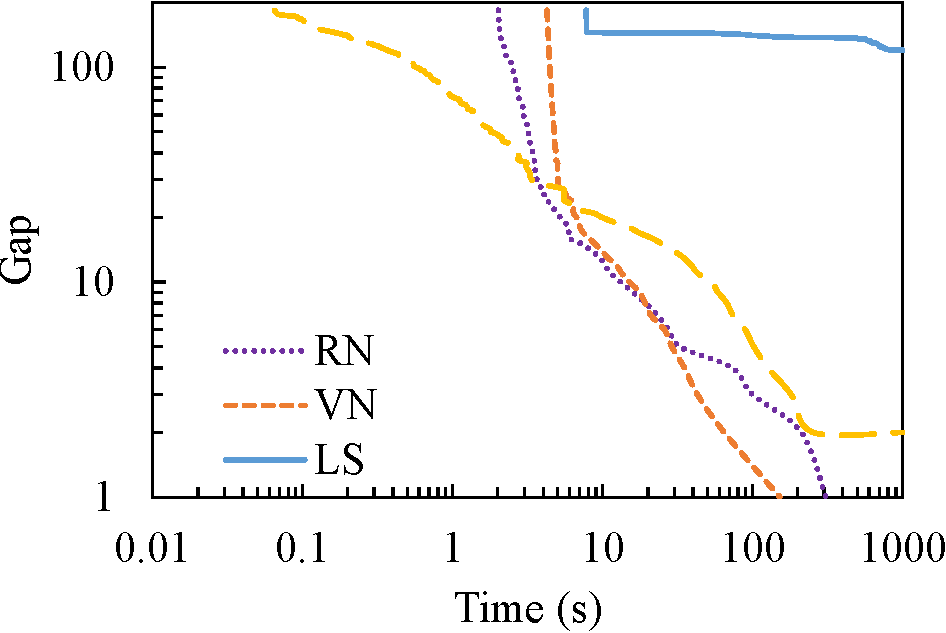
\includegraphics[width=\textwidth]{fig-SampleFigure.pdf}
		\caption{Plot3.}
		\label{fig:convergence3}
	\end{subfigure}
	\caption{Evolution of the objective value gaps again.}
	\label{fig:textwidth}
\end{szxfig*}


\szxrefTab{tab:CmpSOTA} shows ...
\szxreftab{tab:CmpSOTA} shows ...

\begin{szxtab}[!tb]
	\newcommand{\x}[1]{\textbf{#1}}
%	\setlength{\tabcolsep}{1pt}
	\resizebox{\columnwidth}{!}{%
		\begin{tabular}{lrcrrrr}
			\szxtrule
			\multirow{2}{*}{Instance}    & \multicolumn{1}{c}{RefAlg} &  &        \multicolumn{4}{c}{\AlgName{}}        \\
			\szxcrule{2-2}\szxcrule{4-7} &                      Score &  & Score-1h &  Improve &     Score-2h & Improve \\ \szxmrule
			case3                        &                      11610 &  &    11848 &      238 &    \x{11880} &     270 \\
			case4                        &                    2064790 &  &  2071515 &     6725 &  \x{2076537} &   11747 \\
			case5                        &                     699626 &  &   706203 &     6577 &   \x{706860} &    7234 \\
			case6                        &                    2737028 &  &  2743638 &     6610 &  \x{2748924} &   11896 \\
			hidden\_case3                &                      11327 &  &    11520 &      193 &    \x{11554} &     227 \\
			hidden\_case4                &                    2200820 &  &  2206602 &     5782 &  \x{2210688} &    9868 \\
			hidden\_case5                &                     668351 &  &   674361 &     6010 &   \x{676183} &    7832 \\
			hidden\_case6                &                    2785061 &  &  2795109 &    10048 &  \x{2803450} &   18389 \\ \szxmrule
			Total                        &                   11178613 &  & 11220796 &    42183 & \x{11246076} &   67463 \\
			Normalized                   &                    99.62\% &  &        - & 100.00\% &     100.00\% &         \\ \szxbrule
		\end{tabular}%
	}
	\caption{Comparison with the state-of-the-art algorithms.}
	\label{tab:CmpSOTA}
\end{szxtab}

\end{document}
